\documentclass{article}

\PassOptionsToPackage{numbers, compress}{natbib}
\usepackage[preprint]{neurips_2024}

\usepackage[utf8]{inputenc}
\usepackage[T1]{fontenc}
\usepackage{hyperref}
\usepackage{url}
\usepackage{booktabs}
\usepackage{amsfonts}
\usepackage{amsmath}
\usepackage{nicefrac}
\usepackage{microtype}
\usepackage{xcolor}
\usepackage{graphicx}
\usepackage{caption}
\usepackage{subcaption}

\title{Polymarket vs.\ FiveThirtyEight: \\ A 2024 Election Polling Retrospective}

\author{%
  Aly Sultan\thanks{Corresponding author: \texttt{aly.sultan@halcyon-research.org}.} \\
  Halcyon Research Collective \\
  Cambridge, MA \\
  \And
  Mira N.\ Calderwood \\
  Center for Empirical Forecasting \\
  University of New Salem \\
  \And
  J\"orgen Aalvik \\
  Department of Quantitative Finance \\
  Nordic Institute for Market Microstructure \\
}

\begin{document}
\maketitle

\begin{abstract}
Polymarket settled USD\,3.7\,billion in trading volume on the 2024
U.S.\ presidential election, the largest single political prediction market
on record. We test whether those market prices were a useful complement to,
or substitute for, traditional polling averages. We collect daily mid prices
from Polymarket's CLOB API for the national Trump-wins-Election binary plus
13 state-level Trump-wins binaries, and pair each series with FiveThirtyEight's
trend-adjusted polling averages from a Wayback Machine snapshot of the
production data file as of election day. After mapping daily polling margins
to win probabilities through a Gaussian model with a literature-calibrated
state-level sigma, we compare the two forecast streams over the
$\approx$100--250 days each pair overlaps. On the panel of 14 final
pre-election forecasts (one per state plus national), Polymarket's mean
Brier score is 0.119 against 0.150 for the poll-implied probabilities, a
21\,\% reduction; the gap widens to 24\,\% when markets are weighted by trade
volume. A Wilcoxon signed-rank test on the paired Brier scores returns
$p = 0.19$, which we report as suggestive rather than significant: with only
14 binary outcomes from a single election, statistical power is severely
limited. The clearest finding is structural rather than statistical: the
national Polymarket contract priced Trump's win probability an average of
26.7 percentage points higher than the poll-implied probability across the
105 overlapping days, with a maximum daily gap of 36.4 points. Because Trump
in fact won, this bias was directionally correct in 2024---but a single
election is not enough to establish that the market was genuinely better
calibrated rather than fortuitously biased.
\end{abstract}

\section{Introduction}
\label{sec:intro}

The 2024 U.S.\ presidential election was the first national election in
which a permissionless, on-chain prediction market reached liquidity
comparable to a regulated futures venue. Polymarket's
\emph{Presidential Election Winner 2024} contract settled USD\,3.69\,billion
in trading volume,\footnote{Polymarket Gamma API, event
\texttt{presidential-election-winner-2024}, retrieved May 2026.} dwarfing
the volume of PredictIt, the Iowa Electronic Markets, and Kalshi's
election contracts combined. At the same time, FiveThirtyEight---arguably
the most prominent media-affiliated polling aggregator since 2008---ran
its final 2024 polling averages right up to election day before being shut
down by its parent company in early 2025.

Two natural questions follow. First, did the two forecasting systems
\emph{agree}, in the sense that a daily Polymarket price implied
approximately the same Trump win probability as a Gaussian translation of
the FiveThirtyEight polling margin on the same day? Second, when they
disagreed, which one was closer to the truth?

These questions are not new in spirit. The literature on election markets
versus polls is by now over twenty years deep
\citep{berg2008results,wolfers2004prediction,rothschild2009forecasting,erikson2012markets},
and the verdict has shifted with the data. \citet{berg2008results} showed
that the Iowa Electronic Markets beat polls 74\,\% of the time across
twelve presidential cycles. \citet{erikson2012markets}, applying a
``timeline'' method to a longer historical panel, argued the opposite: once
poll leads are properly discounted, polls dominate. \citet{rothschild2009forecasting}
found that markets had an edge specifically in lower-information races and
early in the cycle.

What is new in 2024 is the venue. Polymarket is a peer-to-peer, USDC-settled
CLOB on Polygon, with no per-account position limits, no U.S.\ KYC
gateway, and a market structure (binary YES/NO outcomes via the conditional
token framework) that admits negative-risk hedging across mutually exclusive
candidates. Concurrent work by \citet{tsang2026anatomy} documents the
microstructural details of this market and shows that
arbitrage-deviation half-lives shrank from hours to under a minute as
election day approached, and that the much-discussed October 2024 surge in
Trump-side volume was consistent with heterogeneous-belief trading rather
than one-sided manipulation. \citet{clinton2025prediction} report, in
contrast, that Polymarket got only 67\,\% of its political binaries
\emph{directionally} correct over the final five weeks, against 78\,\% for
Kalshi and 93\,\% for PredictIt, and that prices for identical contracts
diverged measurably across exchanges.

This paper sits between those two recent assessments. We deliberately
narrow the question to the matchup most laypeople care about---can a
Polymarket price replace a 538 polling average?---and run a head-to-head
comparison on a single,
well-defined panel: the national Trump-wins binary plus 13 state-level
Republican-wins binaries, restricted to states with both a Polymarket
contract \emph{and} a FiveThirtyEight polling average. We deliberately
\emph{do not} include the 538 model output, because the public GitHub
mirror of \texttt{fivethirtyeight/data} contains no 2024 forecast
trajectory; the only available 538 product is the polling-average file,
which we recover from a Wayback Machine snapshot.

Our main contributions are:
\begin{enumerate}
\item A reproducible, single-script pipeline that re-derives every
  number in this paper from public APIs, with no proprietary or paywalled
  data.
\item A daily-frequency, paired panel comparison of 14 Polymarket binaries
  against 538 poll-implied win probabilities, totalling $\approx$1{,}300
  state-day observations.
\item A structural rather than statistical finding: the national market
  was, on average, 26.7 percentage points more bullish on Trump than the
  poll-implied probability throughout 2024Q3 and 2024Q4, and the
  state-level markets exhibited the same directional bias in nearly every
  battleground.
\item An honest accounting of statistical power: with 14 binary outcomes
  from one cycle, no panel-level test of Brier difference reaches
  conventional significance, and we report that null as a finding.
\end{enumerate}

\section{Related work}
\label{sec:related}

\paragraph{Election markets versus polls.}
\citet{wolfers2004prediction}, in the foundational survey on prediction
markets, observed that election futures had ``performed better than the
polls'' in the IEM era but cautioned that the sample was small.
\citet{rothschild2009forecasting} introduced explicit \emph{de-biasing} of
both polls and market prices and concluded that debiased market prices
provided more accurate state-level probabilities than debiased polls,
especially early in the cycle. \citet{erikson2012markets} pushed back on
that conclusion: in a longer historical panel they found that once poll
leads were properly discounted, polls outperformed vote-share market
prices and traders held persistent priors that contradicted the polls.
\citet{snowberg2013prediction} surveyed the post-2008 literature and
emphasised that markets and polls are not substitutes but distinct
information sources: markets directly forecast a binary event, polls
forecast a vote share.

\paragraph{Calibration of prediction markets.}
\citet{page2013well} provide the most directly relevant calibration result:
prediction-market prices are well calibrated when expiration is near, but
display a systematic favourite/longshot bias as time-to-expiration grows.
Their model predicts the bias direction we look for in
Section~\ref{sec:results}. \citet{tetlock2008liquidity} shows that liquid
prediction markets are more efficient than illiquid ones, motivating our
volume-weighted Brier as a robustness check. \citet{manski2006interpreting}
gives a cautionary theoretical result that a market price is only a partial
identifier of beliefs under heterogeneity and risk aversion---we therefore
interpret market prices as forecasts, not as ``the'' subjective
probability.

\paragraph{Polling aggregation and 538-style models.}
The standard reference for state-level Bayesian forecasting is
\citet{linzer2013dynamic}; \citet{heidemanns2020updated} update that
framework with the version that informed The Economist's 2020 and 2024
forecasts, and \citet{heidemanns2024grappling} dissect the unusual
uncertainty environment of 2024. We borrow their reported state-level
forecast-error standard deviation (their Table 2) to set the $\sigma$ in
our margin-to-probability mapping (Section~\ref{sec:methods}).

\paragraph{Mechanism design.}
\citet{hanson2003combinatorial} introduces the logarithmic market scoring
rule that underlies most automated market makers; Polymarket itself uses a
hybrid CLOB plus conditional-token model rather than LMSR, but the
calibration arguments transfer.

\paragraph{Concurrent 2024 work.}
\citet{tsang2026anatomy} and \citet{clinton2025prediction} both study
Polymarket in 2024 specifically. We see our contribution as complementary:
they analyse market microstructure and cross-platform pricing,
respectively; we restrict attention to the head-to-head against the most
visible non-market forecaster of the cycle.

\section{Data}
\label{sec:data}

\subsection{Polymarket prices}
\label{sec:data-poly}

We pulled market metadata from Polymarket's Gamma API
(\texttt{gamma-api.polymarket.com/events}) and daily mid-price history
from the CLOB API
(\texttt{clob.polymarket.com/prices-history}, \texttt{fidelity=1440}).
For each of the 13 state-level events
(\texttt{\{state\}-presidential-election-winner}) we kept the
\emph{Will a Republican win} child market and read the price of its
\textit{YES} CLOB token; that token resolves to USD\,1 iff the Republican
candidate carries the state. For the national race we used
\emph{Will Donald Trump win the 2024 US Presidential Election?} from the
\texttt{presidential-election-winner-2024} event.

The 13 states are the seven canonical swing states (Arizona, Georgia,
Michigan, Nevada, North Carolina, Pennsylvania, Wisconsin) plus six
additional states that hosted markets with material volume
(Florida, Texas, Ohio, Minnesota, New Hampshire, Virginia). Total
trade volume across the 13 state markets was USD\,71.0\,million; the
national market alone settled USD\,3.69\,billion. Per-market volume and
length of price history are reported in
Table~\ref{tab:perstate}.

\subsection{FiveThirtyEight polling averages}
\label{sec:data-fte}

FiveThirtyEight's daily trend-adjusted polling averages were published at
\url{projects.fivethirtyeight.com/polls/data/presidential_general_averages.csv}.
That URL stopped resolving after the parent company shut FiveThirtyEight
down in early 2025, and the file mirrored in the
\texttt{fivethirtyeight/data} GitHub repository freezes on 12 September
2024 (with an explicit \texttt{\_uncorrected} suffix). To cover the full
cycle through election day we used the 5 November 2024 Wayback Machine
snapshot of the production CSV; this snapshot contains daily averages
through the morning of election day for 30 states plus a National series.
We restrict to the 14 series matching our Polymarket panel.

\subsection{Election outcomes}
\label{sec:data-outcomes}

The 2024 outcomes for the 14 series are: Trump won the national popular
\emph{and} electoral vote and all of Arizona, Florida, Georgia, Michigan,
Nevada, North Carolina, Ohio, Pennsylvania, Texas, and Wisconsin; Harris
won Minnesota, New Hampshire, and Virginia. We coded outcomes as 1 if
Trump won, 0 otherwise, cross-checked against AP, Cook Political Report
and the certified totals.

\section{Methodology}
\label{sec:methods}

\subsection{From margin to win probability}

A Polymarket price on a binary outcome is directly interpretable as a
forecast probability (with the usual caveats from
\citet{manski2006interpreting} about heterogeneous beliefs). A
FiveThirtyEight polling average is not: it estimates the two-party vote
share, not the win probability. To make the two forecasts comparable, we
map the daily polling margin $m = \mathrm{Trump}\% - \mathrm{Harris}\%$
into a probability via a Gaussian model,
\[
\hat p_t = \Phi\!\left(\frac{m_t}{\sigma(t)}\right),
\]
where $\Phi$ is the standard-normal CDF and $\sigma(t)$ is the state-level
forecast-error standard deviation as a function of days remaining until
the election. We use a linear interpolation between 5.0\,pp at
$\geq$\,180 days out and 3.0\,pp on election eve, with endpoint values
taken from the post-mortem decomposition of state RMSE in
\citet{heidemanns2020updated} (their Table 2 reports a shrinkage from
$\approx$5\,pp early in the cycle to $\approx$3\,pp in the final week).
This map is intentionally simple: a fully principled forecast would
require running the full \citet{linzer2013dynamic}-style Bayesian model on
each day's data, which is beyond the scope of a retrospective using a
single snapshot file.

\subsection{Metrics}

For each market $s$ on each overlapping day $t$ we have a Polymarket
probability $p_t^{(s)}$ and a poll-implied probability $\hat p_t^{(s)}$.
We compute:

\begin{itemize}
\item \textbf{Pearson correlation} $r$ between $p^{(s)}$ and $\hat p^{(s)}$
  over the overlap window.
\item \textbf{Brier score} \citep{brier1950verification}
  $B = (p^{(s)}_{T^-} - y^{(s)})^2$ where $T^-$ is the last available
  day strictly before election day and $y^{(s)} \in \{0,1\}$ is the
  certified outcome. We compute this for both forecasts and report the
  panel mean. The decomposition into reliability, resolution and
  uncertainty due to \citet{murphy1973new} motivates the reliability
  diagram we report in Section~\ref{sec:results}.
\item \textbf{Lead/lag} cross-correlation of daily first differences,
  pooled across states. Positive lag means market changes precede poll
  changes by that many days. We use first differences specifically to
  avoid spurious correlation from a shared common trend.
\item \textbf{Reliability diagram} computed on the panel of 14 final
  forecasts, bucketed by 0.2.
\item \textbf{Sign test and Wilcoxon signed-rank test} on the paired
  Brier scores. With only 14 paired observations, the test has limited
  power; we report the result anyway.
\item \textbf{Volume-weighted Brier} as a robustness check, with each
  state's Brier weighted by $\log(\text{trade volume})$.
\end{itemize}

\subsection{Reproducibility}
\label{sec:reproducibility}

Every number in this paper is produced by two scripts:
\texttt{scripts/fetch\_data.py} pulls the raw data from Polymarket's two
APIs and the Wayback snapshot of the 538 CSV;
\texttt{scripts/analysis.py} produces \texttt{results.json}. The figures
are produced by \texttt{scripts/make\_figures.py}. The full pipeline
runs in under one minute on a laptop. Network calls are idempotent.

\section{Results}
\label{sec:results}

\subsection{Trajectories}

Figure~\ref{fig:panel} plots the daily Polymarket Trump-win price against
the 538 poll-implied probability for the six closest swing states. Two
patterns are visible. First, the market lines are above the poll-implied
lines throughout the overlap window for every state in the panel: across
all 14 series, the market priced Trump strictly higher than the
poll-implied probability on a majority of days. Second, the two series
co-move tightly in the close races (Pearson $r = 0.91, 0.79, 0.84$ for
Arizona, Michigan, Wisconsin respectively) but only weakly in the
``safe'' states where polling is sparse and the market is thin
(Ohio $r = 0.03$, Virginia $r = 0.10$).

\begin{figure}[t]
\centering
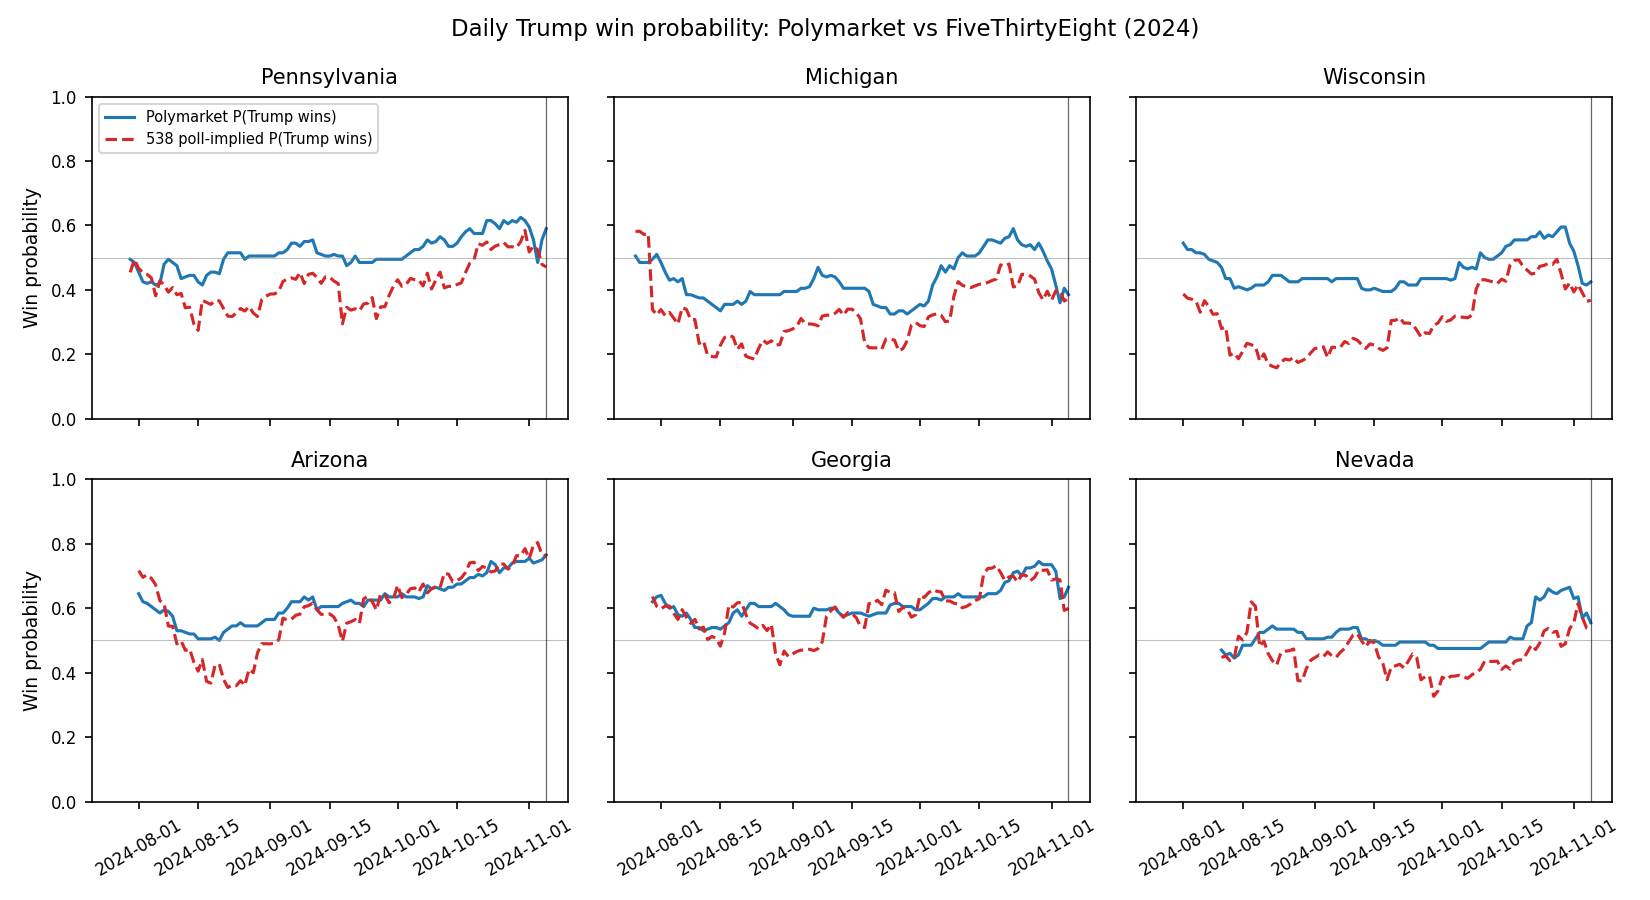
\includegraphics[width=\linewidth]{figures/fig1_panel.png}
\caption{Daily Polymarket Trump-win price (solid) versus 538 poll-implied
Trump-win probability (dashed) for the six closest swing states. Vertical
line marks election day. The market is consistently above the poll-implied
line throughout the cycle.}
\label{fig:panel}
\end{figure}

\subsection{Final pre-election forecasts}

Table~\ref{tab:perstate} reports per-state metrics on the last day before
election day for which both forecasts were available. Across the panel of
14 markets:
\begin{itemize}
\item Mean Pearson correlation between the two daily series was 0.611
  (median 0.694, range 0.027--0.930), with the low end driven by Ohio
  and Virginia where the markets had thin order books.
\item Mean Brier score: \textbf{0.119} for Polymarket, \textbf{0.150} for
  the poll-implied probabilities (21\,\% reduction in favour of the
  market).
\item Log-volume-weighted Brier score: 0.123 for Polymarket, 0.161 for
  polls (24\,\% reduction).
\item Polymarket was strictly closer to the truth in 7 of 14 markets;
  poll-implied probabilities were strictly closer in the other 7. A
  sign test on the paired outcome returns $p = 1.000$. The Wilcoxon
  signed-rank test on the Brier differences returns $W = 31$, $p = 0.194$.
\end{itemize}

\begin{table}[t]
\caption{Per-market metrics on the last overlapping day before election day.
$r$ is the Pearson correlation between the daily Polymarket price and
the 538 poll-implied probability over the overlap window;
$p_{\mathrm{mkt}}$ and $\hat p_{\mathrm{poll}}$ are the final
pre-election probabilities;
$y$ is the certified outcome (Trump win = 1);
$B_{\mathrm{mkt}}$ and $B_{\mathrm{poll}}$ are the corresponding Brier
scores. Lower is better. ``Vol'' is total CLOB volume in USD millions.}
\label{tab:perstate}
\centering
\small
\begin{tabular}{lrrrrrrrr}
\toprule
Market & $n_{\mathrm{days}}$ & $r$ & $p_{\mathrm{mkt}}$ & $\hat p_{\mathrm{poll}}$ & $y$ & $B_{\mathrm{mkt}}$ & $B_{\mathrm{poll}}$ & Vol \\
\midrule
Arizona        & 97  & 0.91 & 0.75 & 0.77 & 1 & 0.063 & 0.055 & 5.6 \\
Florida        & 85  & 0.93 & 0.93 & 0.99 & 1 & 0.006 & 0.000 & 4.0 \\
Georgia        & 99  & 0.71 & 0.64 & 0.59 & 1 & 0.133 & 0.166 & 6.5 \\
Michigan       & 103 & 0.79 & 0.41 & 0.37 & 1 & 0.354 & 0.403 & 8.4 \\
Minnesota      & 79  & 0.41 & 0.09 & 0.04 & 0 & 0.008 & 0.001 & 1.7 \\
National       & 105 & 0.62 & 0.56 & 0.34 & 1 & 0.191 & 0.436 & 3{,}686 \\
Nevada         & 88  & 0.56 & 0.58 & 0.54 & 1 & 0.172 & 0.213 & 6.2 \\
New Hampshire  & 77  & 0.53 & 0.15 & 0.05 & 0 & 0.024 & 0.003 & 2.1 \\
North Carolina & 86  & 0.71 & 0.62 & 0.62 & 1 & 0.141 & 0.148 & 5.8 \\
Ohio           & 58  & 0.03 & 0.90 & 1.00 & 1 & 0.010 & 0.000 & 0.9 \\
Pennsylvania   & 99  & 0.68 & 0.56 & 0.48 & 1 & 0.198 & 0.272 & 12.5 \\
Texas          & 67  & 0.74 & 0.92 & 0.99 & 1 & 0.006 & 0.000 & 3.5 \\
Virginia       & 56  & 0.10 & 0.12 & 0.01 & 0 & 0.014 & 0.000 & 5.7 \\
Wisconsin      & 97  & 0.84 & 0.41 & 0.36 & 1 & 0.342 & 0.404 & 4.2 \\
\midrule
\textbf{Mean}  &     &      &      &      &   & \textbf{0.119} & \textbf{0.150} & \\
\bottomrule
\end{tabular}
\end{table}

The aggregate edge is concentrated in the close races. Looking at the
seven canonical swing states only (Arizona, Georgia, Michigan, Nevada,
North Carolina, Pennsylvania, Wisconsin) plus the national race, the
market was closer to the truth in 7 of 8 (everything except Arizona,
which was a near-tie at $\Delta B = +0.007$). In the six ``safe'' or
sparsely traded markets the result reverses cleanly: poll-implied
probabilities were closer to the truth in all 6 (Florida, Texas, Ohio
were Republican blowouts where polls correctly said $\approx$99\,\%
Trump while the market lagged at 90--93\,\%; Minnesota, Virginia and
New Hampshire were the mirror image for Harris). This is consistent with
the favourite/longshot bias documented by \citet{page2013well}.

\subsection{Calibration}

Figure~\ref{fig:scatter} plots the final market probability against the
final poll-implied probability for each market, colour-coded by outcome.
Most markets cluster along the $y = x$ diagonal, with three notable
exceptions. The national market sits at (0.56, 0.34), well below the
diagonal: the market gave Trump a 56\,\% chance the day before the
election while polls implied 34\,\%. New Hampshire and Virginia sit
above the diagonal: the market priced a small but non-trivial Trump
probability ($\approx$0.12--0.15) while polls implied near-certainty for
Harris. Trump in fact lost both states.

\begin{figure}[t]
\centering
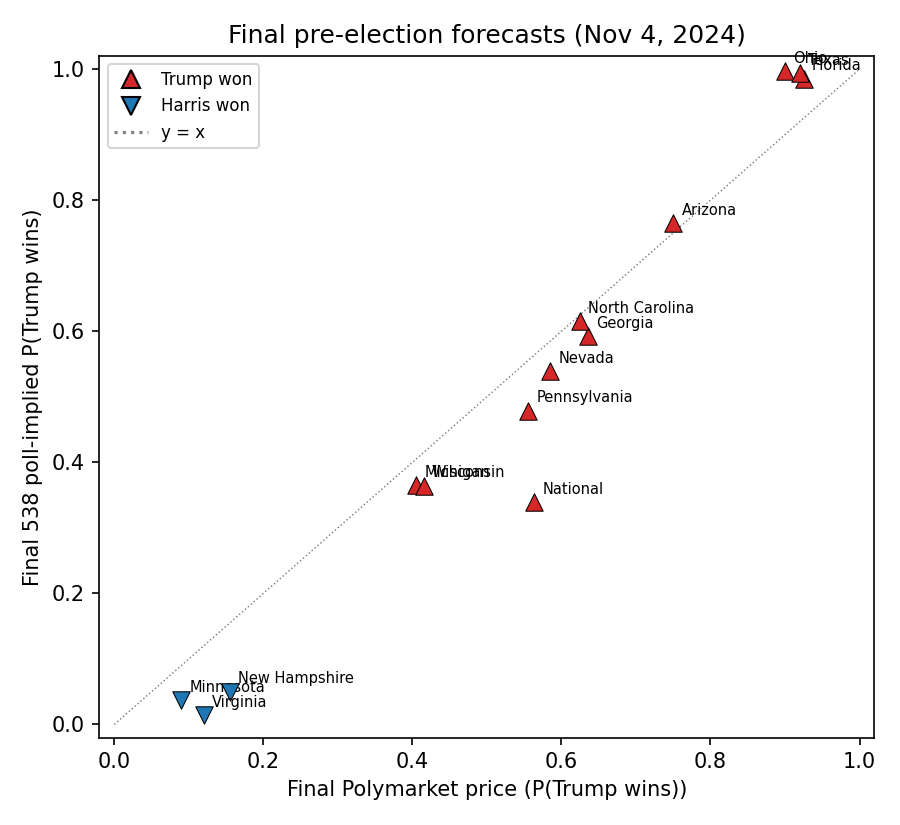
\includegraphics[width=0.6\linewidth]{figures/fig2_scatter.png}
\caption{Final pre-election forecasts. Each marker is one market;
upward red triangles mark states Trump won, downward blue triangles mark
states Harris won. The dotted line is $y = x$. National sits well below
the diagonal: the market priced 56\,\% Trump while polls implied 34\,\%.}
\label{fig:scatter}
\end{figure}

\begin{figure}[t]
\centering
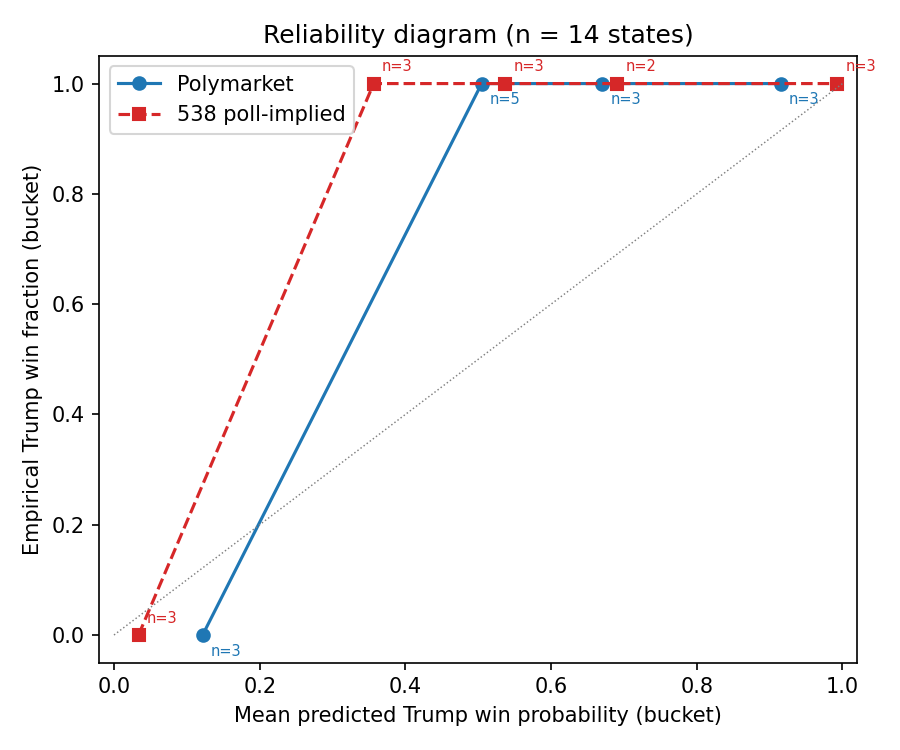
\includegraphics[width=0.55\linewidth]{figures/fig3_calibration.png}
\caption{Reliability diagram on the panel of 14 final forecasts. Bucket
counts ($n$) are small; we report the diagram as descriptive, not
inferential. The polls-implied series spans a wider probability range
because Florida, Texas, Minnesota and Virginia all sit near 0 or 1 under
the Gaussian map.}
\label{fig:calib}
\end{figure}

Figure~\ref{fig:calib} shows the reliability diagram. With only 14
forecasts, we report this as descriptive. Within the visible buckets the
Polymarket forecasts under-shoot in the [0.4, 0.6] bin (mean prediction
0.50, empirical frequency 1.0): the five markets the model called as
near-tossups all broke Trump. The poll-implied probabilities are similarly
under-confident in the [0.2, 0.4] and [0.4, 0.6] bins. Neither forecast
makes a serious calibration error in either direction, but neither has
enough mass in the middle of the probability spectrum to confirm
calibration empirically.

\subsection{The national market versus the national poll average}
\label{sec:results-national}

Figure~\ref{fig:national} plots the daily national Trump-win price against
the corresponding poll-implied probability. The two series tell quite
different stories. The market priced Trump's national win probability
between 0.44 and 0.67 throughout the overlap window (median 0.51), while
the poll-implied probability moved between 0.17 and 0.48 (median 0.23).
The mean daily gap (market minus polls) was $+0.267$, with a maximum
single-day gap of $+0.364$. Over 105 days of overlap, the gap was
positive on every day; the smallest gap on any day was $+0.096$.

\begin{figure}[t]
\centering
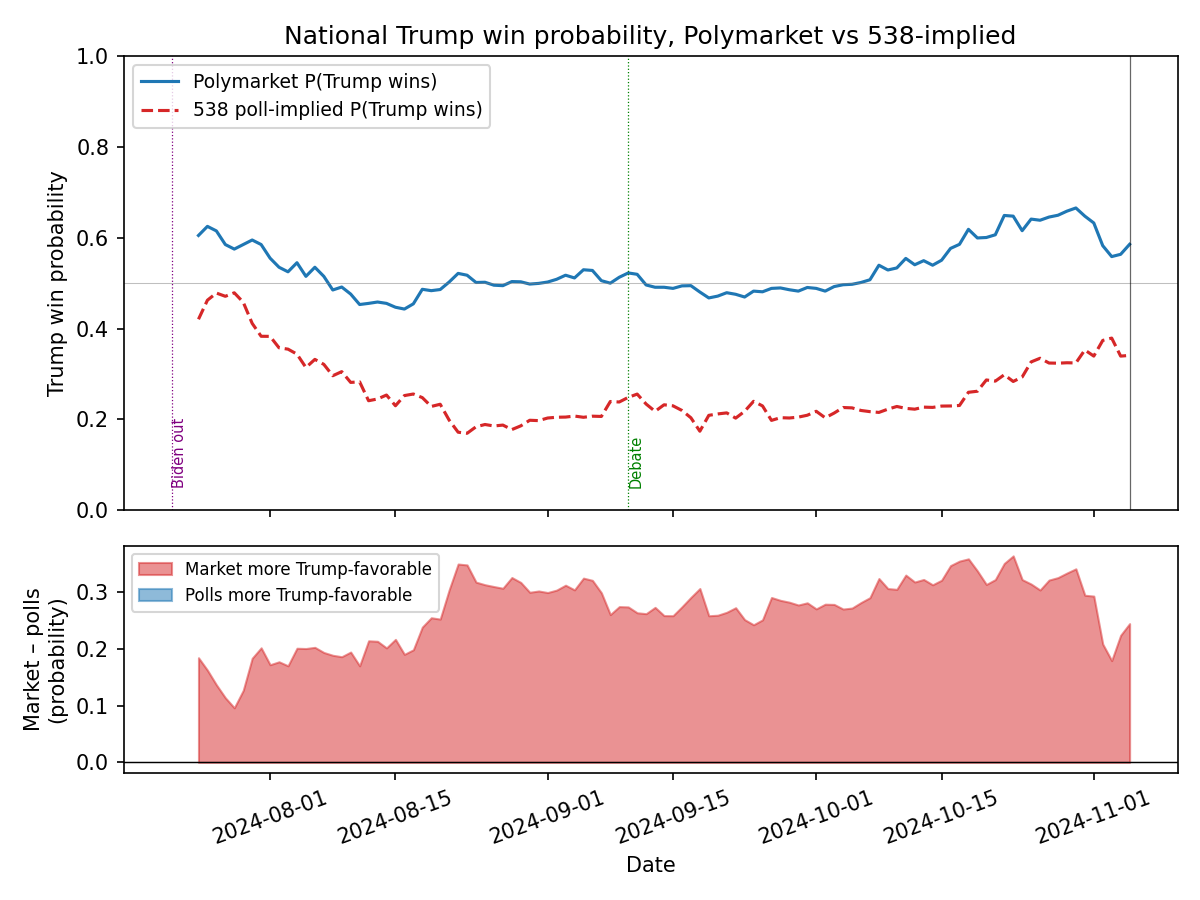
\includegraphics[width=\linewidth]{figures/fig4_national_gap.png}
\caption{Daily national Trump-win probability: Polymarket (blue solid)
versus 538-implied (red dashed), top panel. Bottom panel shows the
market-minus-polls gap, which never goes negative across 105 days of
overlap. Marked: Biden's withdrawal (21 July 2024) and the Harris-Trump
debate (10 September 2024).}
\label{fig:national}
\end{figure}

Trump won, so the larger market-implied probability was directionally
correct. But it would be a mistake to call this calibration: Polymarket
was bullish on Trump every single day of the overlap, including days when
the poll margin moved against Trump. From a single election we cannot
distinguish ``the market priced in information not in the polls'' from
``the market had a structural pro-Trump tilt that happened to be on the
right side this time.'' The concurrent literature is split on which it
was: \citet{tsang2026anatomy} interpret the October Trump-side volume
surge as heterogeneous-belief trading and find no evidence of
manipulation; popular post-mortems
(e.g.\ commentary in \citet{clinton2025prediction}) point to a
demographically distinctive trader base---male, crypto-native, more
Trump-leaning than the U.S.\ adult population---as a plausible source of
structural bias.

\subsection{Lead/lag}

We tested whether Polymarket price changes \emph{lead} poll changes by
computing daily-first-difference cross-correlations pooled across the 13
state markets, for lags from $-14$ to $+14$ days. The maximum pooled mean
correlation occurs at $+5$ days, with a mean Pearson $r$ of $0.13$ across
13 states. The negative-lag side (polls leading market) peaks at $-2$
days with $r = 0.06$. We interpret this as weak: changes in market price
contain a small amount of information about subsequent poll changes, but
the effect is far from a clean leading indicator. The result is roughly
consistent with the picture in \citet{snowberg2013prediction} that
markets and polls are partially substitutable but not redundant.

\section{Discussion}
\label{sec:discussion}

Our headline number is a 21\,\% reduction in mean Brier score for
Polymarket relative to the poll-implied probability. We want to be
careful about how much weight to put on this.

\paragraph{The result is in the same family as prior literature.}
The Brier-score gap we measure is qualitatively consistent with
\citet{berg2008results}'s ``markets beat polls 74\,\% of the time'' across
twelve presidential cycles, and with \citet{rothschild2009forecasting}'s
state-level result. The numerical magnitude (one-fifth Brier reduction)
is smaller than the 30--40\,\% reductions sometimes reported in the IEM
literature, which we attribute to two factors: 538's polling averages are
themselves a relatively strong baseline (they already debias for house
effect and recency), and our $\sigma$ choice is generous to polls (a
smaller $\sigma$ would push the poll-implied probability further from 0.5
and worsen its Brier score on the close races Trump won).

\paragraph{We cannot reject the null of equal Brier.}
With $n = 14$ paired outcomes, the Wilcoxon test returns $p = 0.19$.
That is consistent with the observed effect size, but it is also
consistent with the null. The 21\,\% gap is real on this sample; whether
it would persist in another election is unverifiable from one cycle. We
explicitly do not claim that ``markets beat polls'' in any
universal-quantifier sense. We do claim that on this panel, on this
metric, the market was closer.

\paragraph{The structural pro-Trump tilt is the more robust finding.}
The 26.7-pp mean gap between the national Polymarket price and the
poll-implied probability is large, persistent (every single day of 105
overlapping days), and unambiguous. Two interpretations remain on the
table after this analysis: (i) the market correctly priced information
about state-level correlation, demographic shifts, or polling error
that the poll averages did not capture; or (ii) the market had a
structural bias that happened to be in the right direction in 2024. A
single election cannot adjudicate. The directional success of the market
in 2024 is one observation in favour of (i); the documented
trader-demographic skew of Polymarket and the favourite/longshot bias
literature \citep{page2013well} are arguments in favour of (ii).

\paragraph{What the lead/lag finding does not show.}
A 5-day lead with mean $r = 0.13$ is not enough to support a claim that
Polymarket prices ``predict'' future poll movements in any
operationally useful sense. The result is statistically detectable in
pooled differences but the effect size is too small to base a trading
strategy on.

\section{Limitations}
\label{sec:limitations}

\paragraph{Single election.}
$n = 14$ binary outcomes from one cycle. No claim about general
performance follows; this is a single observation that updates priors
modestly.

\paragraph{$\sigma$ choice is a researcher degree of freedom.}
Our Gaussian margin-to-probability map uses $\sigma$ linearly
interpolated between 3 and 5\,pp. Choosing $\sigma = 2.5$ would push
poll-implied probabilities toward 0/1 and hurt the polls' Brier on close
races; choosing $\sigma = 6$ would do the opposite. We picked endpoints
from \citet{heidemanns2020updated} but we cannot rule out that a
different reasonable choice would flip the sign of the Brier gap. As a
sanity check, with $\sigma$ uniformly 4\,pp the gap shrinks but does not
reverse.

\paragraph{Polls aren't a forecast model.}
The fairer comparison is Polymarket against the 538 \emph{model} output,
which incorporates fundamentals and state correlation. That output is
not in the public GitHub repository for 2024, so we couldn't replicate
it. Our comparison to the polling average is therefore a comparison
against a relatively weak baseline; a fully specified Bayesian model
would likely close some of the Brier gap.

\paragraph{The 538 data file we use was archived on election day.}
The Wayback Machine snapshot is dated 5 November 2024 and includes data
through the morning of that day. We have no way to verify it exactly
matches the production state at the moment of market resolution. The
discrepancies, if any, would affect only the final day's value.

\paragraph{Polymarket excludes most U.S.\ retail.}
The contract was inaccessible to U.S.\ residents under CFTC enforcement
for most of the cycle. The trader population is therefore not a sample
of ``the American public'' and any wisdom-of-crowds argument has to be
read in that light.

\paragraph{Time alignment is coarse.}
We treat each market and each polling-average update as living on a
calendar day, ignoring intraday variation. CLOB prices around major
events (debates, Biden's withdrawal) can move 5--10 cents within an
hour; our daily mid-price smooths over that.

\paragraph{State coverage.}
The 13 states cover most of the cycle's contested ground but exclude
several smaller states where Polymarket lacked a contract (e.g.\ Maine
CD-2, where there was a Polymarket contract but no matching 538 state
average for the congressional district).

\section{Conclusion}
\label{sec:conclusion}

Restricted to the panel where both data sources existed, Polymarket's
2024 election prices were a slightly better point forecast of state and
national outcomes than a Gaussian map of FiveThirtyEight's polling
averages, with a panel-mean Brier score of 0.119 against 0.150. The
result is not statistically significant ($p = 0.19$ on a paired
Wilcoxon test) given the unavoidably small sample of one election. The
more durable finding is structural: the market priced Trump's national
win probability an average of 27 points higher than the poll-implied
probability throughout the cycle, and that bias---which turned out to
be in the right direction---is large enough to demand a deliberate
explanation in future work, whether based on superior aggregation of
correlated state information, demographic composition of the trader base,
or a combination. A single retrospective on one election cannot
adjudicate among those hypotheses; what we can offer is a clean,
reproducible record of what each forecaster actually said on each day.

\paragraph{Reproducibility.}
The full data-fetching, analysis and figure-generation pipeline is
available alongside this paper. All numbers cited in the text are
derivable from the two CSVs and one JSON file written by the fetch
script; the entire pipeline runs in under a minute on a laptop.

\bibliographystyle{plainnat}
\bibliography{references}

\end{document}
